\subsection{Experiment-2. 22.02.2020}\label{experiment-1.-22.02.2020}

The second attempt took place on 22.02.2020.

This time the aim was to check how \textbf{updates} in different parts
of the system behave in real condition:

\begin{itemize}
\tightlist
\item
  a new way to estimate load speed in-app (made an ability to type in IP address from the working app)
\item
  possibility to read app logs right on UE
\item
  improved front-end part (added speed and devices' IDs showing, and so on)
\end{itemize}

The goal did not include a full-scale experiment with as many devices involved, so there were 1 CnC, 1 AP, and 3 UEs with the same settings from the previous experiment but updated app.

The second AP did not participate because of troubles with Wi-Fi access point installation drivers (later update to unstable Debian 11 made it work).

\subsection{Weather conditions}

\begin{itemize}
\tightlist
\item
  no precipitation
\item
  clear sky
\item
  no snow
\item
  strong winds
\end{itemize}

\subsection{Procedure}

Only one case (near-optimal) was performed.

\begin{figure}[H]
	\centering
	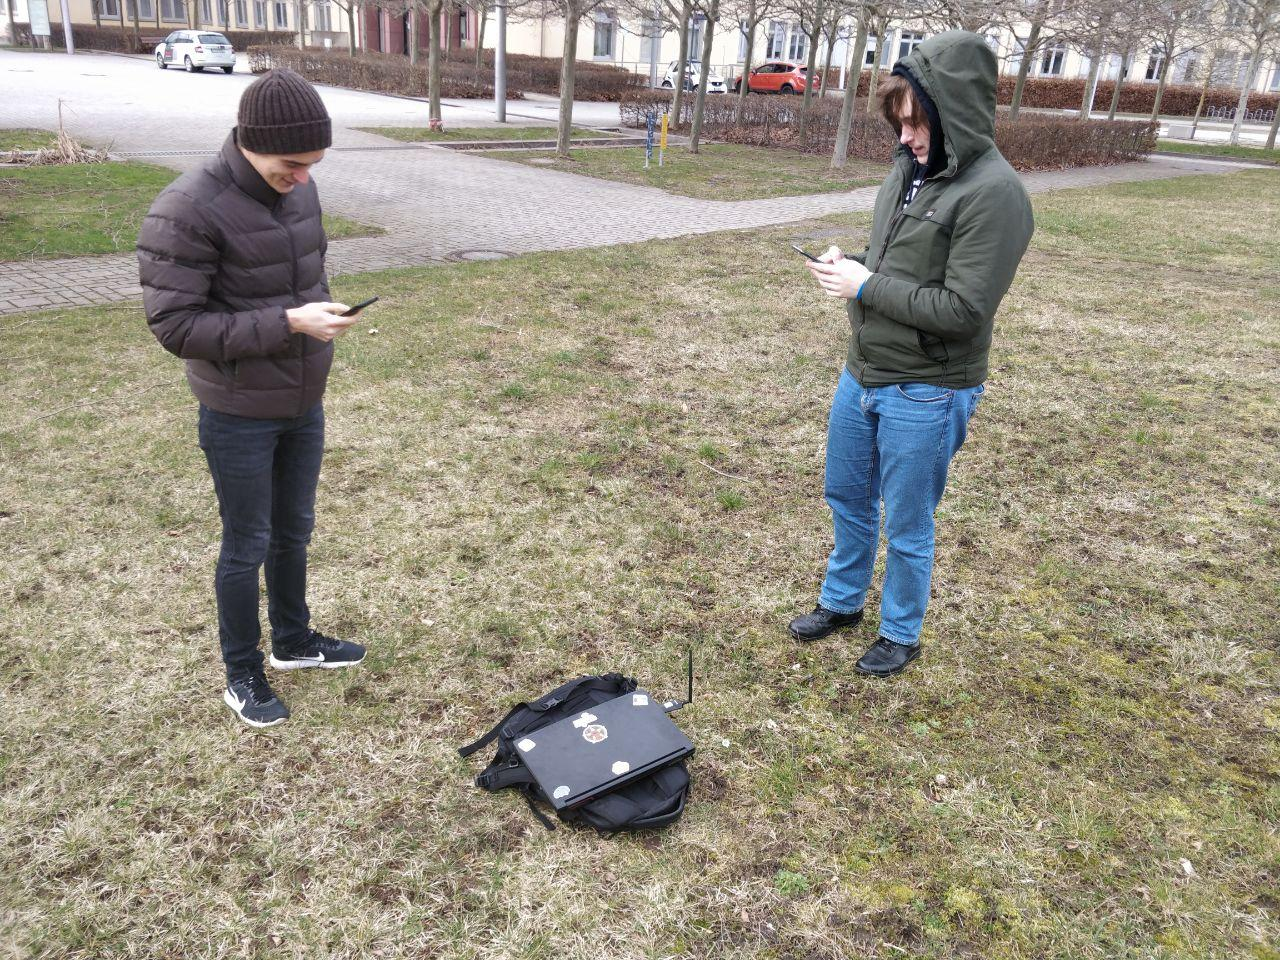
\includegraphics[width=\linewidth,keepaspectratio]{images/experiment_2_overview.jpg}
\caption{The initial CnC server position}
\end{figure}

All the UEs connections made successfully:

\begin{itemize}
\tightlist
\item
  deviceId assigned
\item
  UE coordinates displayed
\end{itemize}

During the first half of the experiment time, after pressing `push once' \textbf{upload/download speeds} were estimated and displayed, although the values seemed to be not realistic (300 000 kBit/s). The values were much smaller when CnC was not connected to the Internet.

Later, pressing 'push once' did not cause speed re-estimation, since the messages from the devices did not reach CnC (lost). Logs did not contain error messages. 

\subsection{Outcome}

The second attempt was also not successful. We hadn't managed to solve the problem in telemetry data sending, some design proposals can be a solution for the next iteration.

As a result, we decided to:

\begin{itemize}
\tightlist
\item
  add logging to APs as well
\item
  implement direct HTTP requests
\end{itemize}
